\documentclass[11pt]{article}
\usepackage{amsmath,amssymb,amsthm,enumerate,tikz, hyperref}
\usetikzlibrary{matrix,arrows}
\usepackage{graphicx}
\usepackage{listings}
%%%%%%%%%%%%%%%%%%%%%%%%%%%%%%%%%%%%%%%%%%%%%%%%%%%%%%%%%%%%%%%
\usepackage{listings}
\definecolor{vertmatlab}{RGB}{28,160,55}
\definecolor{mauvematlab}{RGB}{155,71,239}
\definecolor{lightgray}{gray}{0.5}
\definecolor{IncludeBGround}{RGB}{235,235,235}
\definecolor{listBGround}{RGB}{250,250,250}
%%%%%%%%%%%%%%%%%%%%%%%%%%%%%%%%%%%%%%%%%%%%%%%%%%%%%%%%%%%%%%%%%
\usepackage[usenames,dvipsnames]{color}

% This is the color used for MATLAB comments below
\definecolor{MyDarkGreen}{rgb}{0.0,0.4,0.0}

% For faster processing, load Matlab syntax for listings
\lstloadlanguages{Matlab}%
\lstset{language=Matlab,                        % Use MATLAB
    %frame=single,                           % Single frame around code
    basicstyle=\small\ttfamily,             % Use small true type font
    keywordstyle=\color{blue}\bfseries,        % MATLAB functions bold and blue
    keywordstyle=[2]\color{purple},         % MATLAB function arguments purple
    identifierstyle=\color{purple},
    keywordstyle=[3]\color{Blue}\underbar,  % User functions underlined and blue
    identifierstyle=,                       % Nothing special about identifiers
    % Comments small dark green courier
    commentstyle=\usefont{T1}{pcr}{m}{sl}\color{MyDarkGreen}\small,
    stringstyle=\color{Purple},             % Strings are purple
    showstringspaces=false,                 % Don't put marks in string spaces
    tabsize=5,                              % 5 spaces per tab
    %
    %%% Put standard MATLAB functions not included in the default
    %%% language here
    morekeywords={xlim,ylim,var,alpha,factorial,poissrnd,normpdf,normcdf},
    %
    %%% Put MATLAB function parameters here
    morekeywords=[2]{on, off, interp},
    %
    %%% Put user defined functions here
    morekeywords=[3]{FindESS, homework_example},
    %
    numbers=left,                           % Line numbers on left
    firstnumber=1,                          % Line numbers start with line 1
    numberstyle=\tiny\color{Blue},          % Line numbers are blue
    stepnumber=1                            % Line numbers go in steps of 5
}
%%%%%%%%%%%%%%%%%%%%%%%%%%%%%%%%%%%%%%%%%%%%%%%%%%%%%%%%%%%%%%%%%k
\addtolength{\evensidemargin}{-.5in}
\addtolength{\oddsidemargin}{-.5in}
\addtolength{\textwidth}{0.8in}
\addtolength{\textheight}{0.8in}
\addtolength{\topmargin}{-.4in}
\newtheoremstyle{quest}{\topsep}{\topsep}{}{}{\bfseries}{}{ }{\thmname{#1}\thmnote{ #3}.}
\theoremstyle{quest}
\newtheorem*{definition}{Definition}
\newtheorem*{theorem}{Theorem}
\newtheorem*{question}{Question}
\newtheorem*{subquestion}{Part}
\newtheorem*{exercise}{Exercise}
\newcommand{\subject}{Nonlinear Dynamical Systems}
\newcommand{\name}{James Zoryk.}
\newcommand{\SID}{$\:$2663347.}
\newcommand{\hw}{3}
\newcommand{\ddate}{05.01.2023}
%% If you want to define a new command, you can do it like this:
\newcommand{\Q}{\mathbb{Q}}
\newcommand{\R}{\mathbb{R}}
\newcommand{\Z}{\mathbb{Z}}
\newcommand{\Dp}{\partial}
\newcommand{\Bl}{\mathcal{L}}
\newcommand{\Bll}{\mathcal{L} \left( v , w \right) }

\DeclareMathOperator{\Tr}{Tr}
\DeclareMathOperator{\Det}{Det}
\author{}
\title{\vspace{-50pt}
    \Huge \subject \\ Assignment \hw
\\ \vspace{20pt} \large \name \\ Student Number:\SID}
\date{}
\pagestyle{myheadings}
\markright{\name \SID \hfill Assignment \hw \hfill}



\begin{document}
\maketitle{}

\textbf{Preface:} The matlab files can be accessed and download, along with various 
other documents, via my Github page, which is \href{https://github.com/JamesZor/NLDS_Assignment3}{linked here}.


\begin{question}[1]
\end{question}
\begin{proof}
    Given the following set of PDEs;
    \begin{align*}
        \Dp_t v &= \Dp_{x}^{2} - \gamma v = wv^2, \\
        \Dp_t w &= \beta \Dp_x w +\alpha -w -wv^2.
    \end{align*}
    To find the equilibriums of the given system we set $ \Dp_t w = 0, \Dp_t v = 0$ which yields
    \begin{align*}
        0= v \left( -\gamma + w v \right)\\
        0= \alpha -w -wv^2.
    \end{align*}
    Furthermore, we a bit of work we can compute the 3 equilibriums of the system.
    The fist case to consider is when $v_1 =0$ which implies that $w_1 =\alpha$, hence we have
    $E_1 = \left( 0, \alpha  \right)$. This can be described as the no vegetation state which
    can always exist in the model.

    The other 2 equilibriums arise from when $ wv-\gamma =0$ implies that $v=\gamma / w$, plugging this
    into the second equations gives us $0=w^2 - \alpha w + \gamma^2$. Now using the quadratic equation
    we can solve this to obtain $$ w_{2,3} = \frac{\alpha \pm \sqrt{ \alpha^2 - 4 \gamma }}{2}.$$

    Here we note that if $\alpha < 2 \gamma$, the no vegetation state $E_1$ is the only equilibrium.
    However if it is the case that $ \alpha \geq 2 \gamma$ then we have an addition 2 equilibriums, namely
    $$ E_2 = \left( \frac{\gamma }{w} \, , \frac{1}{2}\left(\alpha + \sqrt{\alpha^2 -4\gamma^2} \right)  \right),
    \quad \text{and} \quad E_3 = \left( \frac{\gamma }{w}\, , \frac{1}{2} \left(\alpha -\sqrt{\alpha^2 -4\gamma^2} \right)  \right). $$
    We observe that $E_2$ is a saddle point and hence is an unstable equilibrium point for the model.
    Lastly for $E_3$ we see that the determinate of the Jacobian matrix is give as
    \begin{align*}
        J_{E_3} = 
        \begin{bmatrix}
            2vw - \gamma & v^2 \\
            -2vw & -1 -v^2 \\
        \end{bmatrix}
        .
    \end{align*}
    Here it can be shown that $\Det(J_{E_3}) > 0$ so then the stability is determined by the trace $\Tr(J_{E_3})$.
    Moreover, we observe that $\Tr(J_{E_3}) = 0$ along the curve given by $\alpha = \frac{\gamma^2}{\sqrt{\gamma-1}}$, given
    $\gamma > 1$. This can be seen in the mathematica note book found on Github.
\end{proof}
\clearpage

\begin{question}[2]
    Linerised 
\end{question}
\begin{proof}
    \begin{align*}
        \Dp_t
        \begin{bmatrix}
            \tilde{v} \\
            \tilde{w} \\
        \end{bmatrix}  = 
        \mathcal{L} \left( v_*, w_* \right)
        \begin{bmatrix}
            \tilde{v} \\
            \tilde{w} \\
        \end{bmatrix}   
    \end{align*}
    Here we define $\mathcal{L} = \left[ \frac{\Dp f_i }{ \Dp u_j } \right]$ for $i$ and $j=1,2$. 
    Computing this yields the following matrix 
    \begin{align*}
        \mathcal{L} \left( v_*, w_* \right)  &=
        \begin{bmatrix}
            \frac{d}{dv} v & \frac{d}{dw} v \\
            \frac{d}{dv} w & \frac{d}{dw} w \\
        \end{bmatrix} \\
        &=
        \begin{bmatrix}
            \Dp_{x}^{2} - \gamma + 2 w_* v_* & {v_*}^2 \\
            -2w_* v_* & \beta \Dp_x -1 - {v_*}^2 \\
        \end{bmatrix}
        .
    \end{align*}
\end{proof}
\clearpage
\begin{question}[3]
    Perturbation of the vegetative equilibrium. 
\end{question}
\begin{proof}
    Using the expression $\gamma = v_* w_*$ which was found in part A we can simplify $\Bl$
    to 
    \begin{align*}
        \Bl =
        \begin{bmatrix}
            \Dp_x^2 + \gamma & v_*^2\\
            - 2\gamma & \beta \Dp_x -1  -v_*^2
        \end{bmatrix}.
    \end{align*}
    Now using the derivates $$\Dp_x = \frac{d}{dx}( \varphi(x,t) ) = \frac{d}{dx} \exp{ \left( \lambda t+ i k x  \right)  } = ik$$ 
    and $$ \Dp_x^2 = -k^2$$ 
    yields the following expression
    \begin{align*}
        \Bl =
        \begin{bmatrix}
            -k^2 + \gamma & v_*^2\\
            - 2\gamma & i\beta k  -1  -v_*^2
        \end{bmatrix}
        .
    \end{align*}
    Using the equilibrium expression for $E_3$ we have $v_* = \gamma/ w_*$, then it follows that
    \begin{align*}
        \frac{\gamma}{w_3} &= \frac{ 2 \gamma }{(\alpha - \sqrt{ \alpha^2 - 4 \gamma^2 })} \\
                           &= \frac{2 \gamma (\alpha + \sqrt{ \alpha^2 - 4 \gamma^2 })}{(\alpha - \sqrt{ \alpha^2 - 4 \gamma^2 })(\alpha + \sqrt{ \alpha^2 - 4 \gamma^2 })} \\
                           &= \frac{ 2 \gamma (\alpha + \sqrt{ \alpha^2 - 4 \gamma^2 }) }{4\gamma^2} \\
                           &= \frac{(\alpha + \sqrt{ \alpha^2 - 4 \gamma^2 }) }{2 \gamma} \\ 
                           &= \mu(\alpha, \gamma).
    \end{align*}
    Hence we have
    \begin{align*}
        \Bl =
        \begin{bmatrix}
            -k^2 + \gamma & \mu^2\\
            - 2\gamma & i\beta k  -1  -\mu^2
        \end{bmatrix}
    \end{align*}
    as required.
\end{proof}
\clearpage
\begin{question}[4]
    Dispersion Relation. 
\end{question}
\begin{proof}
    For both $\lambda$ of the Jacobian matrix we plot the real and imaginary parts for the 
    parameters $(8,20,2)$, which can be seen in $\ref{fig:q4fig1}$. In which we observe
    $\Re(\lambda_2) < 0 $, implies that the equilibrium is stable. The can also be extended
    to $\Re(\lambda_1) < 0$ which is not shown in the plot. 
    Moreover we see in both cases $\Im(\lambda_1)$ and $\Im(\lambda_2)$ are not constant functions
    which implies there is a circle motion in the stream plot. However, we also observe
    that the they are not the complex conjugate of each other.
    Hence the vegetative equilibrium is linear stable for $(8,20,2)$.
    \begin{figure}[h!]
        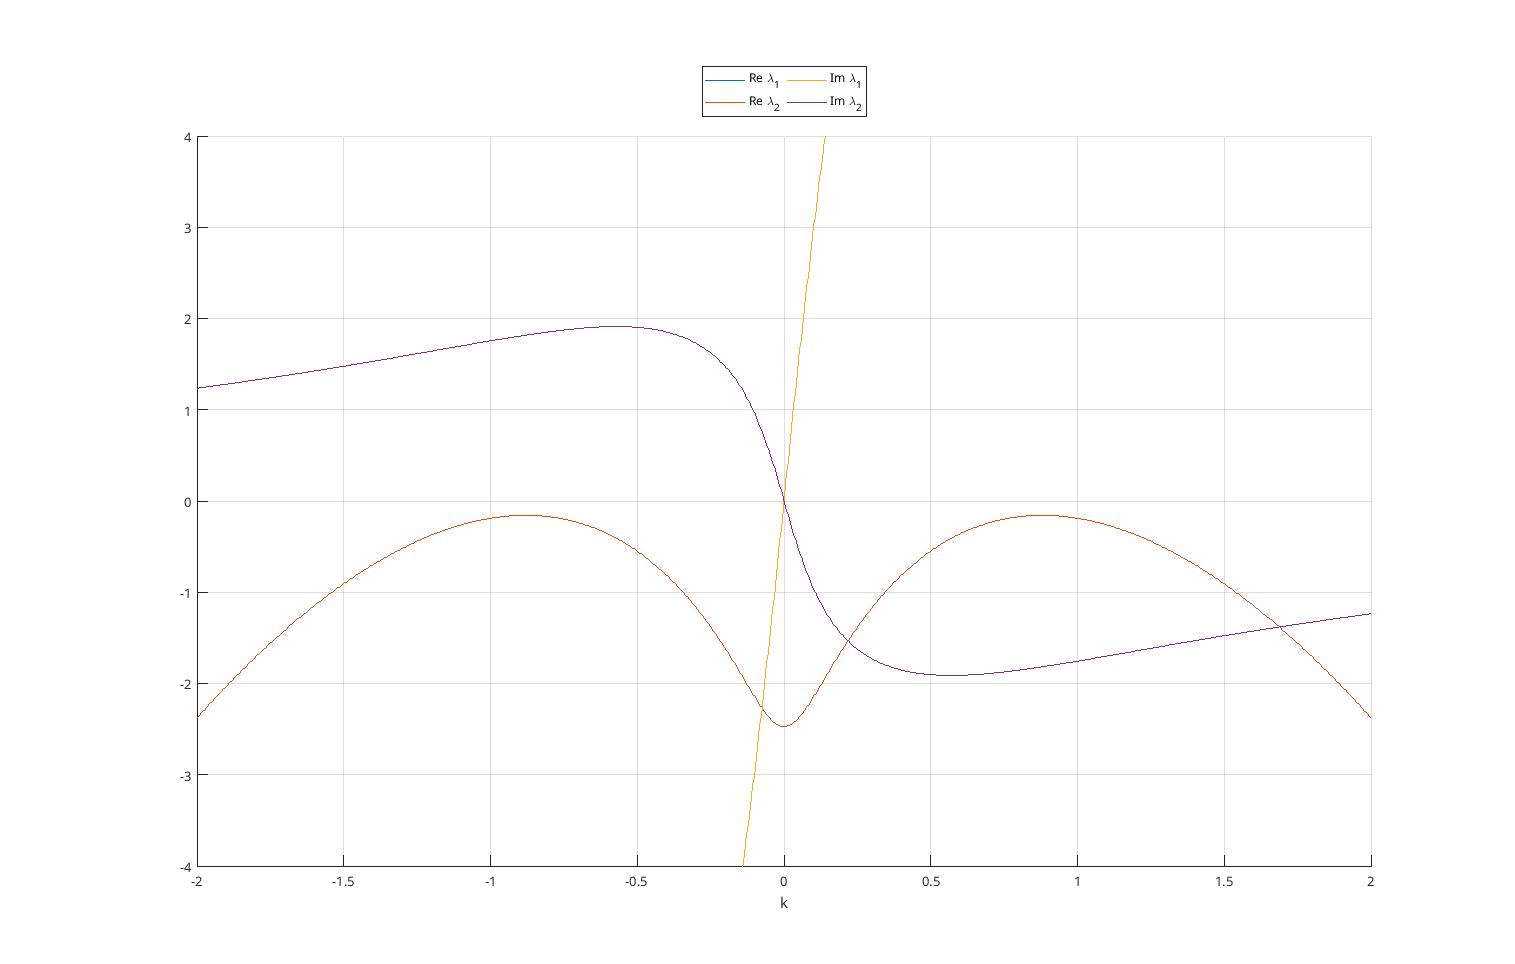
\includegraphics[width=\linewidth]{figures/Q4_fig1.jpg}
        \caption{The graph of $\lambda_1$ and $\lambda_2$ with both the real and imaginary parts
        plot with the parameters of $ \alpha = 8, \beta = 20 $ and $2$.}
        \label{fig:q4fig1}
    \end{figure}

    \lstinputlisting[language=matlab]{code/A3Question4.m} 

\end{proof}
\clearpage
\begin{question}[5]
   Pattern-forming instability. 
\end{question}
\begin{proof}
    We can observe numerically from Figure $\ref{fig:q5fig1}$ that $\Re( \lambda_2 (k, 8) ) < 0 $ so that it is a stable equilibrium 
    and that $\Re( \lambda_2 (k, 7) ) > 0$ which implies that it is an unstable equilibrium.
    
    Moreover, it can be shown that the function $\Re( \lambda_2 (k, \alpha) )$ is continuous for values of
    $\alpha = [7,8]$, since $\lambda_2$ is a polynomial function. Hence by the Intermediate value theorem
    there must exits an $\alpha_* \in [7,8] $ and $k_*$ such that $\Re( \lambda_2 (k_*, \alpha_* ) ) = 0$. 
    Namely that $\alpha_*$ is a critical value.

    We see that for $\alpha \leq \alpha_*$ there emerges a propagating wave pattern instability.
    This is since there exist both $\pm k_*$ such that $\Re(\lambda(\pm k_* , \alpha_*)) =0 $ while 
    also we have $\Im(\lambda_2(\pm k_* , \alpha_*)) \neq 0$.
    
    Hence we can compute the wave length by $ \Delta = 2 \pi / k_*$ so in the case when $\alpha =7$ 
    we can use matlab to numerically find $k_* = 0.8038$ which yields a wave length of $ \Delta = 7.8166$.
    The speed of the propagating is computed by $ c = - \Im(\lambda_*) / k_*$, here $\lambda_*$ is the maximum
    value that the $\lambda$ function obtains. In the case of $\alpha =7$ we have
    $\Im(\lambda_*)= -1.6169$, thus we have a travelling wave speed of $c = 2.0115$.

    \begin{figure}[h!]
        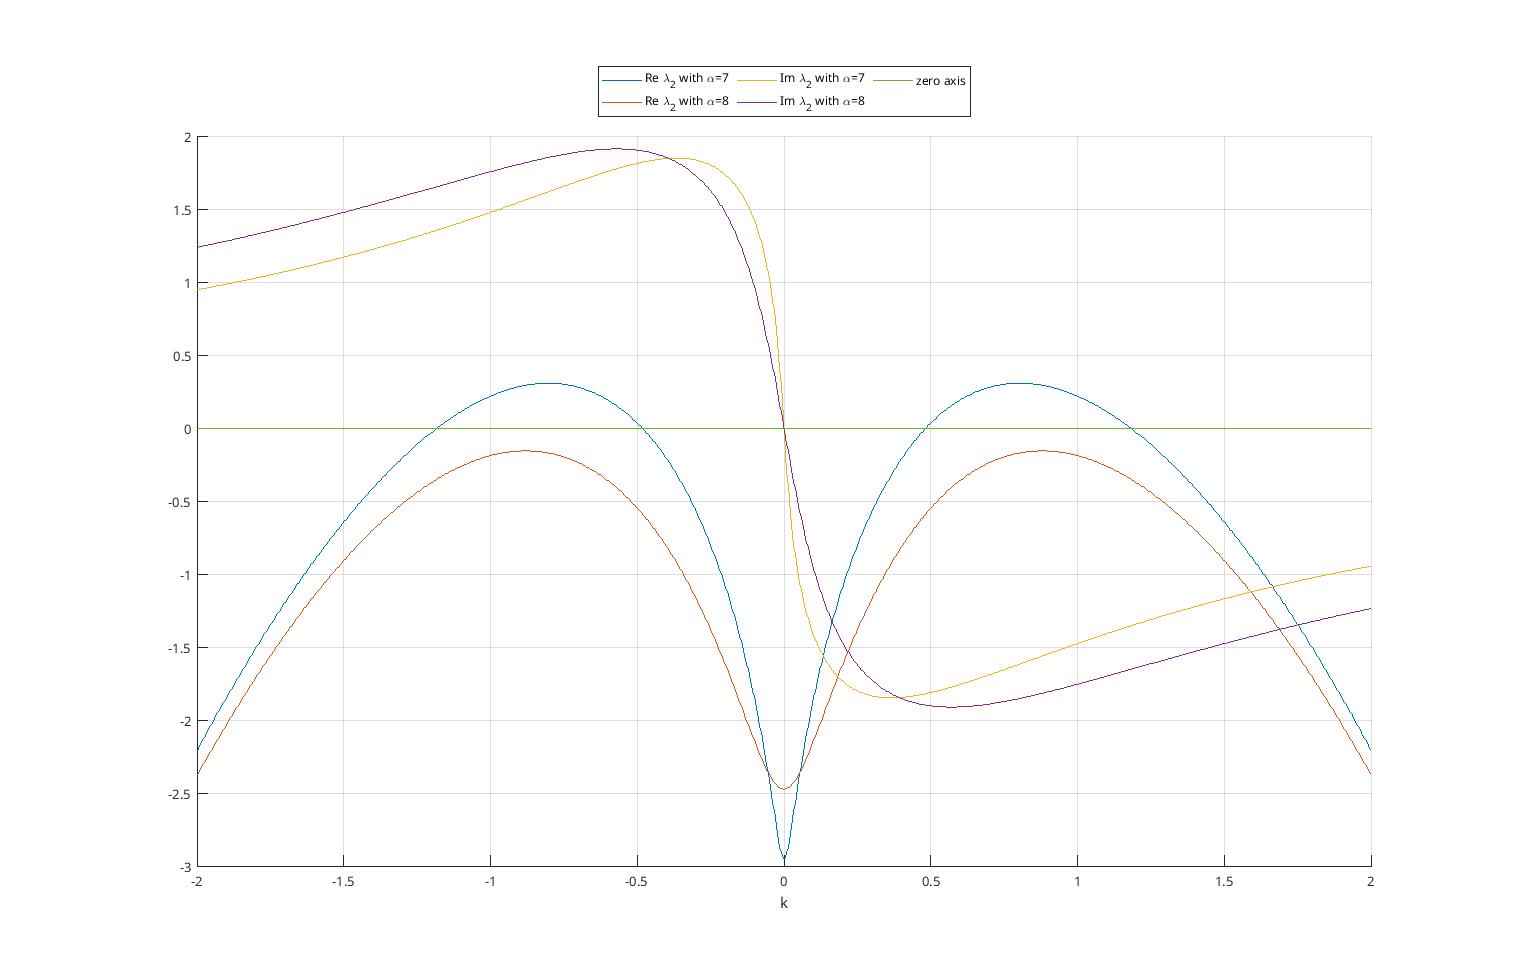
\includegraphics[width=\linewidth]{figures/Q5_fig1.jpg}
        \caption{Graphical plots of real and imaginary parts of $\lambda_2 (k)$ for parameters $\alpha=[7,8]$,
        $\beta =20$ and $\gamma =2$.}
        \label{fig:q5fig1}
    \end{figure}

    \lstinputlisting[language=matlab]{code/A3Question5.m} 
    
\end{proof}
\clearpage

\begin{question}[6]
    
\end{question}
\begin{proof}
    For this question we fix the parameters to $(7,20,2)$, while we apply the Periodic boundary
    conditions with setting $L=15.7$ and the initial conditions of
    \begin{align*}
        \begin{pmatrix}
            v(x,0) \\ w(x,0)
        \end{pmatrix}
        =
        \begin{pmatrix}
            v_{*,3} \\ w_{*,3}
        \end{pmatrix}
        +
        \begin{pmatrix}
            \cos{ \left( 4 \pi x / L \right)  } \\ 1
        \end{pmatrix}.
    \end{align*}
    Using numerically methods and matlab we can obtain the following plots, which shows
    the existence of a propagating wave. In Figure $\ref{fig:q6fig2}$ we see that peaks of the
    waves occur at $x_1 = 8.52$ and $x_2= 0.6908$, which gives $\Delta = | x_1 - x_2 | = 7.8292$.
    We see this value is close to the one computed in Question 5, which confirms our findings.
    Moreover, we also observe that in Figure $\ref{fig:q6fig1}$ that we have a dialogical lines,
    namely that we have periodic in both $x$ and $t$, this implies that there exists a propagating
    wave, which we computed as in  Question 5.
    \begin{figure}[h!]
        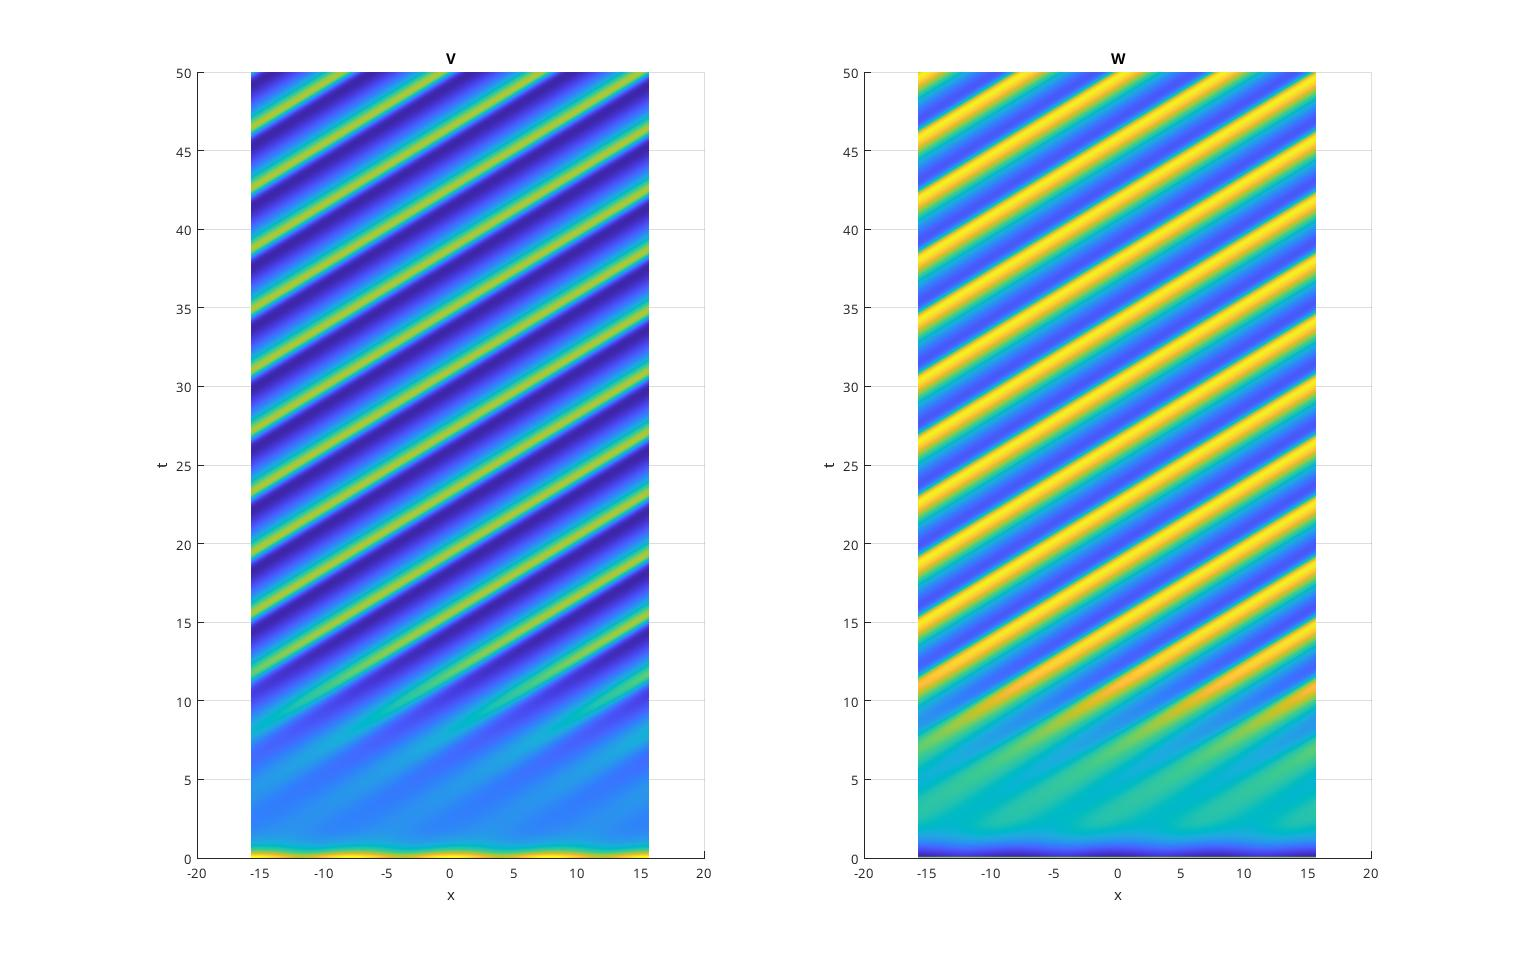
\includegraphics[width=\linewidth]{figures/Q6_fig1.jpg}
        \caption{3D plot of the tiger bush Pattern-forming, in time, space and density.
        For parameters $(7,20,2)$, $L=15.7$.}
        \label{fig:q6fig1}
    \end{figure}
    \begin{figure}[h!]
        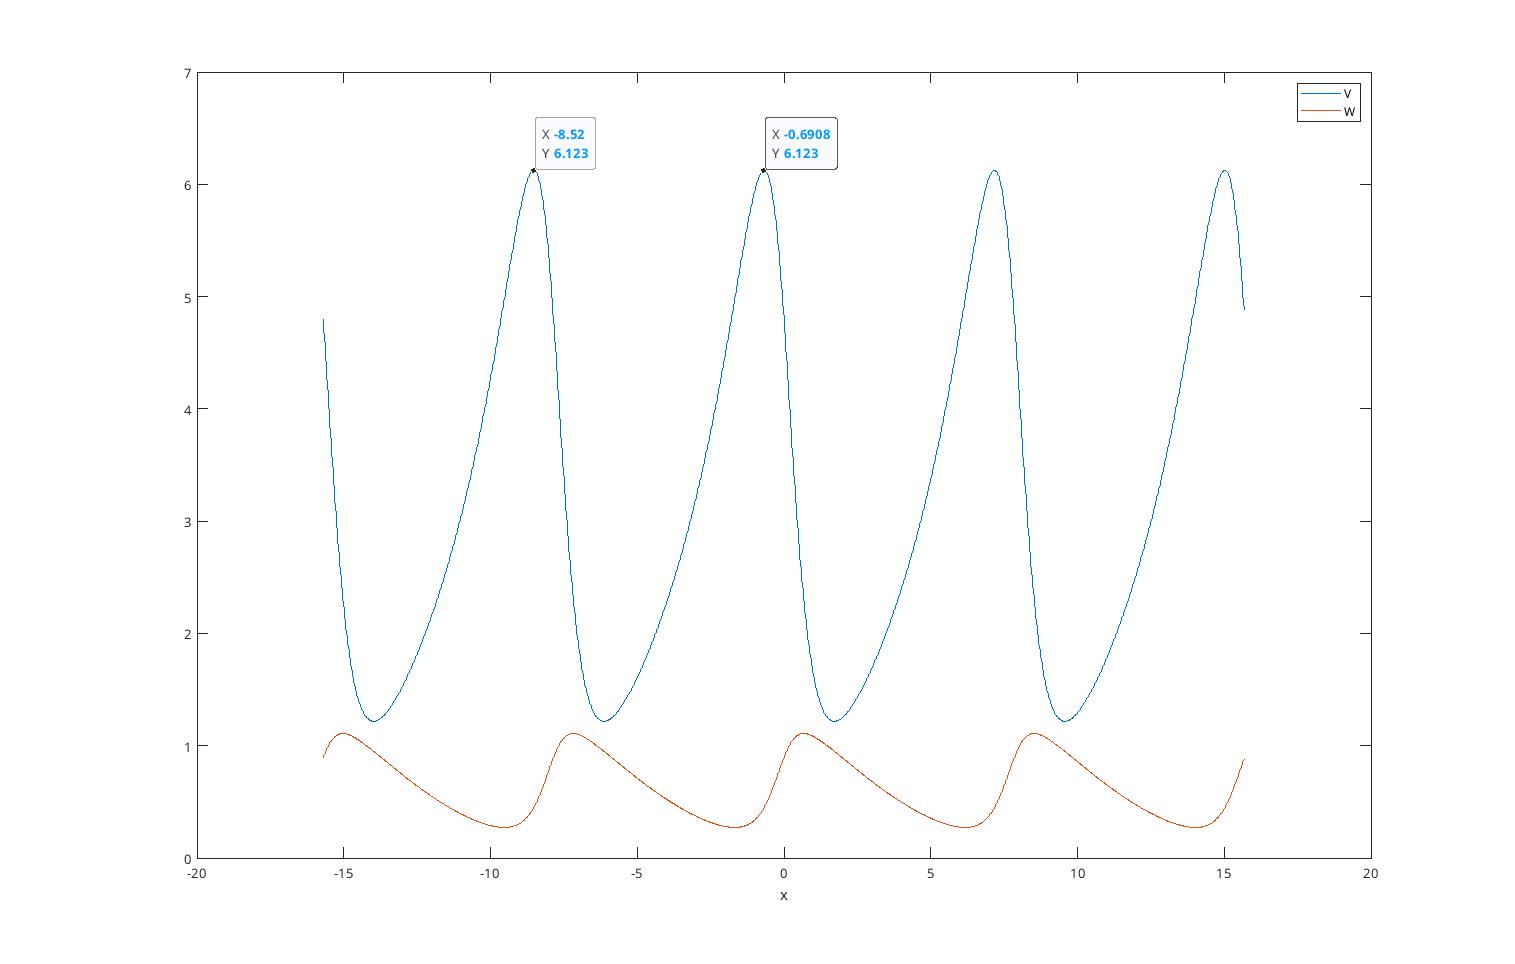
\includegraphics[width=\linewidth]{figures/Q6_fig2.jpg}
        \caption{Wave shapes of the Tiger bush pattern. Here we also mark two consecutive peaks
        in order to measure the wave length. For parameters $(7,20,2)$, $L=15.7$.}
        \label{fig:q6fig2}
    \end{figure}
    \clearpage
    \lstinputlisting[language=matlab]{code/A3Question6.m} 
\end{proof}
\end{document}
